%% \VignetteIndexEntry{CSSP: ChIP-Seq Statistical Power}
\documentclass[a4paper,10pt]{article}
\usepackage{amsmath,mathrsfs,graphicx}
\usepackage[top=2cm,bottom=2cm,left=2cm,right=2cm]{geometry}
\usepackage[utf8]{inputenc}
\usepackage{hyperref}
\usepackage{color}
%\usepackage{natbib}

\title{atSNP: affinity tests for regulatory SNP detection}

\author{Chandler Zuo\footnote{Department of Statistics and of Biostatistics and Medical Informatics, 1300 University Avenue, Madison, WI, 53706, USA.}\\
Sunyoung Shin\footnote{Department of Statistics and of Biostatistics and Medical Informatics, 1300 University Avenue, Madison, WI, 53706, USA.}  \\
S\"und\"uz Kele\c{s}\footnote{Departments of Statistics and of Biostatistics and Medical Informatics, 1300 University Avenue, Madison, WI, 53706, USA.}}
  
\date{}

\usepackage{Sweave}
\begin{document}
\maketitle

\tableofcontents

\section{Introduction}

This document provides an introduction to the affinity test for large sets of SNP-motif interactions using the \texttt{atSNP} package(\textbf{a}ffinity \textbf{t}est for regulatory \textbf{SNP} detection) \cite{zuo14}. \texttt{atSNP} implements in-silico methods for identifying SNPs that potentially may affect binding affinity of transcription factors. Given a set of SNPs and a library of motif position weight matrices (PWMs), \texttt{atSNP} provides three main functions for analyzing SNP effects:

\begin{enumerate}
\item Computing the binding affinity score for each allele and each PWM;
\item Computing the p-values for allele-specific binding affinity scores;
\item Computing the p-values for affinity score changes between the two alleles for each SNP.
\end{enumerate}

\texttt{atSNP} implements the importance sampling algorithm in \cite{isample} to compute the p-values. Compared to other bioinformatics tools, such as FIMO \cite{fimo} and is-rSNP \cite{is-rsnp}, that provides similar functionalities, \texttt{atSNP} avoides computing the p-values analytically. This reduces the execution time drastically because the probability sample space is a exponential order of the motif length. In one of our research projects, we have used atSNP to evaluate interactions between 26K SNPs and 2K motifs within 5 hours. We found no other existing tool can finish the analysis of such a scale.

\section{Installation}

We are working to make the package available through bioconductor. The developing version can be installed from the Github repository:

\begin{Schunk}
\begin{Sinput}
> library(devtools)
> install_github("chandlerzuo/atSNP")
\end{Sinput}
\end{Schunk}

The following dependent \texttt{R} packages are required:

\begin{itemize}
\item \texttt{data.table} is used for formatting results that are easy for users to query;
\item \texttt{motifStack} is relied upon to draw sequence logo plots;
\item \texttt{doMC} is used for parallel computation;
\item \texttt{Rcpp} interfaces the C++ codes that implements the importance sampling algorithm;
\item \texttt{testthat} is used for unit testing.
\end{itemize}
  
In addition, users also need to install the annotation package from \url{www.bioconductor.org/packages/3.0/data/annotation/} that corresponds to the species type and genome version. Our example SNP data set in the subsequent sections corresponds to the hg19 version of human genome. To repeat the sample codes in this vignette, the \texttt{BSgenome.Hsapiens.UCSC.hg19} package is required.

\section{Example}

\subsection{Load motif and SNP data}

\texttt{atSNP} provdes a default motif library downloaded from \url{compbio.mit.edu/encode-motifs/motifs.txt}. This library contains 2065 known and discovered motifs from ENCODE TF ChIP-seq data sets. The following commands allow you to load this motif library:

\begin{Schunk}
\begin{Sinput}
> library(atSNP)
> data(encode_motif)
> length(motif_encode)
\end{Sinput}
\begin{Soutput}
[1] 2065
\end{Soutput}
\begin{Sinput}
> motif_encode[seq(3)]
\end{Sinput}
\begin{Soutput}
$SIX5_disc1
             [,1]       [,2]     [,3]        [,4]
 [1,] 8.51100e-03 4.2550e-03 0.987234 1.00000e-10
 [2,] 9.02127e-01 1.2766e-02 0.038298 4.68090e-02
 [3,] 4.55319e-01 7.2340e-02 0.344681 1.27660e-01
 [4,] 2.51064e-01 8.5106e-02 0.085106 5.78724e-01
 [5,] 1.00000e-10 4.6809e-02 0.012766 9.40425e-01
 [6,] 1.00000e-10 1.0000e-10 1.000000 1.00000e-10
 [7,] 3.82980e-02 2.1277e-02 0.029787 9.10638e-01
 [8,] 9.44681e-01 4.2550e-03 0.051064 1.00000e-10
 [9,] 1.00000e-10 1.0000e-10 1.000000 1.00000e-10
[10,] 1.00000e-10 1.0000e-10 0.012766 9.87234e-01

$MYC_disc1
             [,1]        [,2]        [,3]        [,4]
 [1,] 1.73516e-01 1.05023e-01 7.21461e-01 1.00000e-10
 [2,] 1.00000e-10 1.00000e-10 1.00000e-10 1.00000e+00
 [3,] 1.00000e-10 1.00000e+00 1.00000e-10 1.00000e-10
 [4,] 1.00000e+00 1.00000e-10 1.00000e-10 1.00000e-10
 [5,] 1.00000e-10 9.58904e-01 1.00000e-10 4.10960e-02
 [6,] 5.93610e-02 1.00000e-10 9.40639e-01 1.00000e-10
 [7,] 1.00000e-10 1.00000e-10 1.00000e-10 1.00000e+00
 [8,] 1.00000e-10 1.00000e-10 1.00000e+00 1.00000e-10
 [9,] 1.00000e+00 1.00000e-10 1.00000e-10 1.00000e-10
[10,] 1.00000e-10 7.26028e-01 1.14155e-01 1.59817e-01

$SRF_disc1
             [,1]  [,2]  [,3]        [,4]
 [1,] 1.00000e-10 1e+00 1e-10 1.00000e-10
 [2,] 1.00000e-10 1e+00 1e-10 1.00000e-10
 [3,] 4.95495e-01 1e-10 1e-10 5.04505e-01
 [4,] 2.61261e-01 1e-10 1e-10 7.38739e-01
 [5,] 1.00000e+00 1e-10 1e-10 1.00000e-10
 [6,] 1.00000e-10 1e-10 1e-10 1.00000e+00
 [7,] 7.29730e-01 1e-10 1e-10 2.70270e-01
 [8,] 5.04505e-01 1e-10 1e-10 4.95495e-01
 [9,] 1.00000e-10 1e-10 1e+00 1.00000e-10
[10,] 1.00000e-10 1e-10 1e+00 1.00000e-10
\end{Soutput}
\end{Schunk}

The data object 'encode\_motif' also contains a character vector 'motif\_info' that contains detailed information for each motif:

\begin{Schunk}
\begin{Sinput}
> length(motif_info)
\end{Sinput}
\begin{Soutput}
[1] 2065
\end{Soutput}
\begin{Sinput}
> head(motif_info)
\end{Sinput}
\begin{Soutput}
                                                SIX5_disc1 
  "SIX5_GM12878_encode-Myers_seq_hsa_r1:MEME#1#Intergenic" 
                                                 MYC_disc1 
  "USF2_K562_encode-Snyder_seq_hsa_r1:MDscan#1#Intergenic" 
                                                 SRF_disc1 
 "SRF_H1-hESC_encode-Myers_seq_hsa_r1:MDscan#2#Intergenic" 
                                                 AP1_disc1 
    "JUND_K562_encode-Snyder_seq_hsa_r1:MEME#1#Intergenic" 
                                                SIX5_disc2 
"SIX5_H1-hESC_encode-Myers_seq_hsa_r1:MDscan#1#Intergenic" 
                                                 NFY_disc1 
    "NFYA_K562_encode-Snyder_seq_hsa_r1:MEME#2#Intergenic" 
\end{Soutput}
\end{Schunk}

Users can also provide a list of PWMs as the motif library via the 'LoadMotifLibrary' function. In this function, 'tag' specifies the string that marks the start of each block of PWM; 'skiprows' is the number of description lines before the PWM; 'skipcols' is the number of columns to be skipped in the PWM matrix; 'transpose' is TRUE if the PWM has 4 rows representing A, C, G, T or FALSE if otherwise; 'field' is the position of the motif name within the description line; 'sep' is a vector of separators in the PWM; 'pseudocount' is the number added to the raw matrices, recommended to be 1 if the matrices are in fact position frequency matrices. These arguments provide the flexibility of loading a number of varying formatted files. The PWMs are returned as a list object. This function flexibly adaps to a variety of different formats. Some examples using online accessible files from other research groups are shown below.

\begin{Schunk}
\begin{Sinput}
> pwms <- LoadMotifLibrary(
+  "http://meme.nbcr.net/meme/examples/sample-dna-motif.meme-io")
> pwms <- LoadMotifLibrary(
+  "http://compbio.mit.edu/encode-motifs/motifs.txt",
+  tag = ">", transpose = FALSE, field = 1, 
+  sep = c("\t", " ", ">"), skipcols = 1, 
+  skiprows = 1, pseudocount = 0)
> pwms <- LoadMotifLibrary(
+  "http://johnsonlab.ucsf.edu/mochi_files/JASPAR_motifs_H_sapiens.txt",
+  tag = "/NAME",skiprows = 1, skipcols = 0, transpose = FALSE,
+  field = 2)
> pwms <- LoadMotifLibrary(
+  "http://jaspar.genereg.net/html/DOWNLOAD/ARCHIVE/JASPAR2010/all_data/matrix_only/matrix.txt", 
+  tag = ">", skiprows = 1, skipcols = 1, transpose = TRUE, 
+  field = 1, sep = c("\t", " ", "\\[", "\\]", ">"),
+  pseudocount = 1)
> pwms <- LoadMotifLibrary(
+  "http://jaspar.genereg.net/html/DOWNLOAD/JASPAR_CORE/pfm/nonredundant/pfm_vertebrates.txt",
+  tag = ">", skiprows = 1, skipcols = 0, transpose = TRUE, field = 1, 
+  sep = c(">", "\t", " "), pseudocount = 1)
> pwms <- LoadMotifLibrary(
+  "http://gibbs.biomed.ucf.edu/PreDREM/download/nonredundantmotif.transfac", 
+  tag = "DE", skiprows = 1, skipcols = 1, 
+  transpose = FALSE, field = 2, sep = "\t")
\end{Sinput}
\end{Schunk}

The data set for the SNP information must be a table including five columns:

\begin{itemize}
\item chr: the chromosome ID;
\item snp: the genome coordinate of the SNP;
\item snpid: the string for the SNP name;
\item a1, a2: nucleotides for the two alleles at the SNP position.
\end{itemize}
  
This data set can be loaded using the 'LoadSNPData' function. The 'genome.lib' argument specifies the annotation package name corresponding to the SNP data set, with the default as 'BSgenome.Hsapiens.UCSC.hg19'. Each side of the SNP is extended by a number of base pairs specified by the 'half.window.size' argument. 'LoadSNPData' extracts the genome sequence within such windows around each SNP using the 'genome.lib' package. An example is the following:


'LoadSNPData' simultaneously estimates the parameters for the first order Markov model in the reference genome using the nucleotides within the SNP windows. It returns a list object with five fields:

\begin{itemize}
\item \$sequence\_matrix: a matrix with (2$\times$'half.window.size' + 1), with each column corresponding to one SNP. The entries 1-4 represent the A, C, G, T nucleotides;
\item \$ref\_base: a vector coding the reference allele nucleotides for all SNPs;
\item \$snp\_base: a vector coding the SNP allele nucleotides for all SNPs;
\item \$prior: the stationary distribution parameters for the Markov model;
\item \$transition: the transition matrix for the first order Markov model.
\end{itemize}

A toy sample data set including a preloaded motif library and a SNP set is included in the package:

\begin{Schunk}
\begin{Sinput}
> data(example)
> names(motif_library)
\end{Sinput}
\begin{Soutput}
[1] "SIX5_disc1" "MYC_disc1"  "SRF_disc1"  "AP1_disc1"  "SIX5_disc2"
[6] "ALX3_2"     "AFP_1"     
\end{Soutput}
\begin{Sinput}
> str(snpInfo)
\end{Sinput}
\begin{Soutput}
List of 5
 $ sequence_matrix: int [1:61, 1:1997] 4 3 1 4 3 2 2 1 3 3 ...
  ..- attr(*, "dimnames")=List of 2
  .. ..$ : NULL
  .. ..$ : chr [1:1997] "rs10910078" "rs4486391" "rs3748816" "rs2843401" ...
 $ ref_base       : int [1:1997] 4 1 1 4 4 4 4 1 1 4 ...
 $ snp_base       : int [1:1997] 2 4 3 2 2 2 2 2 3 2 ...
 $ transition     : num [1:4, 1:4] 0.317 0.354 0.292 0.214 0.177 ...
  ..- attr(*, "dimnames")=List of 2
  .. ..$ : chr [1:4] "A" "C" "G" "T"
  .. ..$ : chr [1:4] "A" "C" "G" "T"
 $ prior          : Named num [1:4] 0.289 0.207 0.207 0.297
  ..- attr(*, "names")= chr [1:4] "A" "C" "G" "T"
\end{Soutput}
\begin{Sinput}
> ## to look at the motif information
> data(encode_motif)
> motif_info[names(motif_library)]
\end{Sinput}
\begin{Soutput}
                                                SIX5_disc1 
  "SIX5_GM12878_encode-Myers_seq_hsa_r1:MEME#1#Intergenic" 
                                                 MYC_disc1 
  "USF2_K562_encode-Snyder_seq_hsa_r1:MDscan#1#Intergenic" 
                                                 SRF_disc1 
 "SRF_H1-hESC_encode-Myers_seq_hsa_r1:MDscan#2#Intergenic" 
                                                 AP1_disc1 
    "JUND_K562_encode-Snyder_seq_hsa_r1:MEME#1#Intergenic" 
                                                SIX5_disc2 
"SIX5_H1-hESC_encode-Myers_seq_hsa_r1:MDscan#1#Intergenic" 
                                                    ALX3_2 
                                     "ALX3_jolma_DBD_M449" 
                                                     AFP_1 
                                    "AFP1_transfac_M00616" 
\end{Soutput}
\end{Schunk}


\subsection{Affinity score tests}

The binding affinity scores for all pairs of SNP and PWM can be computed by the 'ComputeMotifScore' function. It returns a list of two fields: 'snp.tbl' is a data.table containing the nucleotide sequences for each SNP; 'motif.scores' is a data.table containing the binding affinity scores for each SNP-motif pair.

\begin{Schunk}
\begin{Sinput}
> motif_score <- ComputeMotifScore(motif_library, snpInfo, ncores = 2)
> motif_score$snp.tbl
\end{Sinput}
\begin{Soutput}
           snpid                                                       ref_seq
   1: rs10910078 TGATGCCAGGTGGTCAGTGGGTTTTTGCCATCCGCCAGGAGCTTCACTGGGCCTCCCGTTG
   2:  rs4486391 ATGGAGAATTCCACAGCTGATTGGAACCTAAACGAGAGAACCAAATGGACATCCCAGGGCT
   3:  rs3748816 TTGGAGTACTCCTCGTCCAGGCGCCTGTTCATCTCCTCCAGGATGTAGTCAGGGTGCCCGA
   4:  rs2843401 TCCTCCACCATTGTGCCAAACAGCGCCTGGTGGGGCCACCCGATCATCCCACGGGCCCCCA
   5:  rs2843402 CACCTTCTGGGCTGCAGGACTTCCTGCCCTTTAGGAAAGGGAGGCAGCCCTTTCTTCCTCC
  ---                                                                         
1993:  rs3003207 CACCAAAACAGCTATGTCATTTTAGAAATGCAAATTGGACCCTAGAGTTTGATTATCAGCA
1994:  rs1173830 ATATAATCTATTCTTTCTTTCCCTTTCCTTCTCCAGAAACAGCTCAAATTATGAAATAACT
1995:   rs654873 GCTTCAGTAAAATTAACATTGATGAGTACCCTTATGGAATCTATCATGCATGTTCCAATTT
1996:  rs1768071 GGTGTCAGGGAATGCCAATCTCGCTGGTTCCGGTTTATTAGCTCGGGGAATCTCGTTAGAT
1997:  rs1538961 CTACCAGGTGCCAGTTGAGGATAGTCTAAACTACATTCTCAGCTTGAAATATTTTTGACCA
                                                            snp_seq
   1: TGATGCCAGGTGGTCAGTGGGTTTTTGCCACCCGCCAGGAGCTTCACTGGGCCTCCCGTTG
   2: ATGGAGAATTCCACAGCTGATTGGAACCTATACGAGAGAACCAAATGGACATCCCAGGGCT
   3: TTGGAGTACTCCTCGTCCAGGCGCCTGTTCGTCTCCTCCAGGATGTAGTCAGGGTGCCCGA
   4: TCCTCCACCATTGTGCCAAACAGCGCCTGGCGGGGCCACCCGATCATCCCACGGGCCCCCA
   5: CACCTTCTGGGCTGCAGGACTTCCTGCCCTCTAGGAAAGGGAGGCAGCCCTTTCTTCCTCC
  ---                                                              
1993: CACCAAAACAGCTATGTCATTTTAGAAATGTAAATTGGACCCTAGAGTTTGATTATCAGCA
1994: ATATAATCTATTCTTTCTTTCCCTTTCCTTTTCCAGAAACAGCTCAAATTATGAAATAACT
1995: GCTTCAGTAAAATTAACATTGATGAGTACCTTTATGGAATCTATCATGCATGTTCCAATTT
1996: GGTGTCAGGGAATGCCAATCTCGCTGGTTCTGGTTTATTAGCTCGGGGAATCTCGTTAGAT
1997: CTACCAGGTGCCAGTTGAGGATAGTCTAAATTACATTCTCAGCTTGAAATATTTTTGACCA
                                                        ref_seq_rev
   1: CAACGGGAGGCCCAGTGAAGCTCCTGGCGGATGGCAAAAACCCACTGACCACCTGGCATCA
   2: AGCCCTGGGATGTCCATTTGGTTCTCTCGTTTAGGTTCCAATCAGCTGTGGAATTCTCCAT
   3: TCGGGCACCCTGACTACATCCTGGAGGAGATGAACAGGCGCCTGGACGAGGAGTACTCCAA
   4: TGGGGGCCCGTGGGATGATCGGGTGGCCCCACCAGGCGCTGTTTGGCACAATGGTGGAGGA
   5: GGAGGAAGAAAGGGCTGCCTCCCTTTCCTAAAGGGCAGGAAGTCCTGCAGCCCAGAAGGTG
  ---                                                              
1993: TGCTGATAATCAAACTCTAGGGTCCAATTTGCATTTCTAAAATGACATAGCTGTTTTGGTG
1994: AGTTATTTCATAATTTGAGCTGTTTCTGGAGAAGGAAAGGGAAAGAAAGAATAGATTATAT
1995: AAATTGGAACATGCATGATAGATTCCATAAGGGTACTCATCAATGTTAATTTTACTGAAGC
1996: ATCTAACGAGATTCCCCGAGCTAATAAACCGGAACCAGCGAGATTGGCATTCCCTGACACC
1997: TGGTCAAAAATATTTCAAGCTGAGAATGTAGTTTAGACTATCCTCAACTGGCACCTGGTAG
                                                        snp_seq_rev
   1: CAACGGGAGGCCCAGTGAAGCTCCTGGCGGGTGGCAAAAACCCACTGACCACCTGGCATCA
   2: AGCCCTGGGATGTCCATTTGGTTCTCTCGTATAGGTTCCAATCAGCTGTGGAATTCTCCAT
   3: TCGGGCACCCTGACTACATCCTGGAGGAGACGAACAGGCGCCTGGACGAGGAGTACTCCAA
   4: TGGGGGCCCGTGGGATGATCGGGTGGCCCCGCCAGGCGCTGTTTGGCACAATGGTGGAGGA
   5: GGAGGAAGAAAGGGCTGCCTCCCTTTCCTAGAGGGCAGGAAGTCCTGCAGCCCAGAAGGTG
  ---                                                              
1993: TGCTGATAATCAAACTCTAGGGTCCAATTTACATTTCTAAAATGACATAGCTGTTTTGGTG
1994: AGTTATTTCATAATTTGAGCTGTTTCTGGAAAAGGAAAGGGAAAGAAAGAATAGATTATAT
1995: AAATTGGAACATGCATGATAGATTCCATAAAGGTACTCATCAATGTTAATTTTACTGAAGC
1996: ATCTAACGAGATTCCCCGAGCTAATAAACCAGAACCAGCGAGATTGGCATTCCCTGACACC
1997: TGGTCAAAAATATTTCAAGCTGAGAATGTAATTTAGACTATCCTCAACTGGCACCTGGTAG
\end{Soutput}
\begin{Sinput}
> motif_score$motif.scores[, list(snpid, motif, log_lik_ref,
+                                 log_lik_snp, log_lik_ratio)]
\end{Sinput}
\begin{Soutput}
            snpid     motif log_lik_ref log_lik_snp log_lik_ratio
    1: rs10910078     AFP_1  -117.69581  -116.93812    -0.7576857
    2:  rs4486391     AFP_1   -73.54122   -95.18078    21.6395566
    3:  rs3748816     AFP_1   -73.94669   -96.74940    22.8027074
    4:  rs2843401     AFP_1  -139.33536  -141.41480     2.0794415
    5:  rs2843402     AFP_1   -95.07542   -95.40392     0.3285041
   ---                                                           
13975:  rs3003207 SRF_disc1   -72.43032   -73.11450     0.6841775
13976:  rs1173830 SRF_disc1   -93.09039   -93.09039     0.0000000
13977:   rs654873 SRF_disc1   -93.09039   -70.39764   -22.6927498
13978:  rs1768071 SRF_disc1  -116.44934  -115.83145    -0.6178913
13979:  rs1538961 SRF_disc1   -96.14035   -73.11450   -23.0258509
\end{Soutput}
\end{Schunk}

The affinity scores for the reference and the SNP alleles are represented by the 'log\_lik\_ref' and 'log\_lik\_snp' columns in '\$motif.scores'. The affinity score change is included in the 'log\_lik\_ratio' column. These three affinity scores are tested in the subsequent steps. '\$motif.scores' also include other columns for the position of the best matching subsequence on each allele. For a complete description on all these columns, users can look up the help documentation.

After we have computed the binding affinity scores, they can be tested using the 'ComputePValues' function. The result is a data.table extending the affinity score table by three columns: 'pval\_ref' is the p-value for the reference allele affinity score; 'pval\_snp' is the p-value for the SNP allele affinity score; and 'pval\_diff' is the p-value for the affinity score change between the two alleles.

\begin{Schunk}
\begin{Sinput}
> motif.scores <- ComputePValues(motif.lib = motif_library,
+                                snp.info = snpInfo,
+                                motif.scores = motif_scores$motif.scores,
+                                ncores = 7)
> motif.scores[, list(snpid, motif, pval_ref, pval_snp, pval_diff)]
\end{Sinput}
\begin{Soutput}
            snpid     motif  pval_ref   pval_snp  pval_diff
    1: rs10910078     AFP_1 0.9776495 0.96265483 0.77254685
    2:  rs4486391     AFP_1 0.3767000 0.76858447 0.25680145
    3:  rs3748816     AFP_1 0.4267265 0.90817363 0.08460265
    4:  rs2843401     AFP_1 0.9911095 0.99822551 0.58550863
    5:  rs2843402     AFP_1 0.7636040 0.80776942 0.86817355
   ---                                                     
13975:  rs3003207 SRF_disc1 0.2372302 0.24653492 0.66522050
13976:  rs1173830 SRF_disc1 0.2673992 0.26739919 1.00000000
13977:   rs654873 SRF_disc1 0.2618610 0.05817295 0.25026857
13978:  rs1768071 SRF_disc1 0.7770457 0.69299844 0.68555718
13979:  rs1538961 SRF_disc1 0.6604981 0.24653492 0.03966129
\end{Soutput}
\end{Schunk}

\subsection{Additional analysis}

atSNP provides additional functions to extract the matched nucleotide subsequences that match to the motifs. Function 'MatchSubsequence' adds the subsequence matches to the affinity score table by using the motif library and the SNP set. The subsequences matching to the motif in the two alleles are returned in the 'ref\_match\_seq' and 'snp\_match\_seq' columns. The 'IUPAC' column returns the IUPAC letters of the motifs. Notice that if you have a large number of SNPs and motifs, the returned table can be very large.

\begin{Schunk}
\begin{Sinput}
> match_result <- MatchSubsequence(snp.tbl = motif_scores$snp.tbl,
+                                  motif.scores = motif.scores,
+                                  motif.lib = motif_library,
+                                  snpids = c("rs10910078", "rs4486391"),
+                                  motifs = names(motif_library)[1:2],
+                                  ncores = 2)
> match_result[, list(snpid, motif, IUPAC, ref_match_seq, snp_match_seq)]
\end{Sinput}
\begin{Soutput}
        snpid      motif      IUPAC ref_match_seq snp_match_seq
1: rs10910078  MYC_disc1 GTCACGTGAC    GGCGGATGGC    GCCACCCGCC
2: rs10910078 SIX5_disc1 GARWTGTAGT    CTGGCGGATG    GGCGGGTGGC
3:  rs4486391  MYC_disc1 GTCACGTGAC    TAAACGAGAG    CTCGTATAGG
4:  rs4486391 SIX5_disc1 GARWTGTAGT    CTCGTTTAGG    CTCGTATAGG
\end{Soutput}
\end{Schunk}

We can also visualize how each motif is matched to each allele using the 'plotMotifMatch' function:

\begin{Schunk}
\begin{Sinput}
> plotMotifMatch(snp.tbl = motif_scores$snp.tbl,
+                motif.scores = motif_scores$motif.scores,
+                snpid = motif_scores$snp.tbl$snpid[50],
+                motif.lib = motif_library,
+                motif = motif_scores$motif.scores$motif[1])
\end{Sinput}
\end{Schunk}
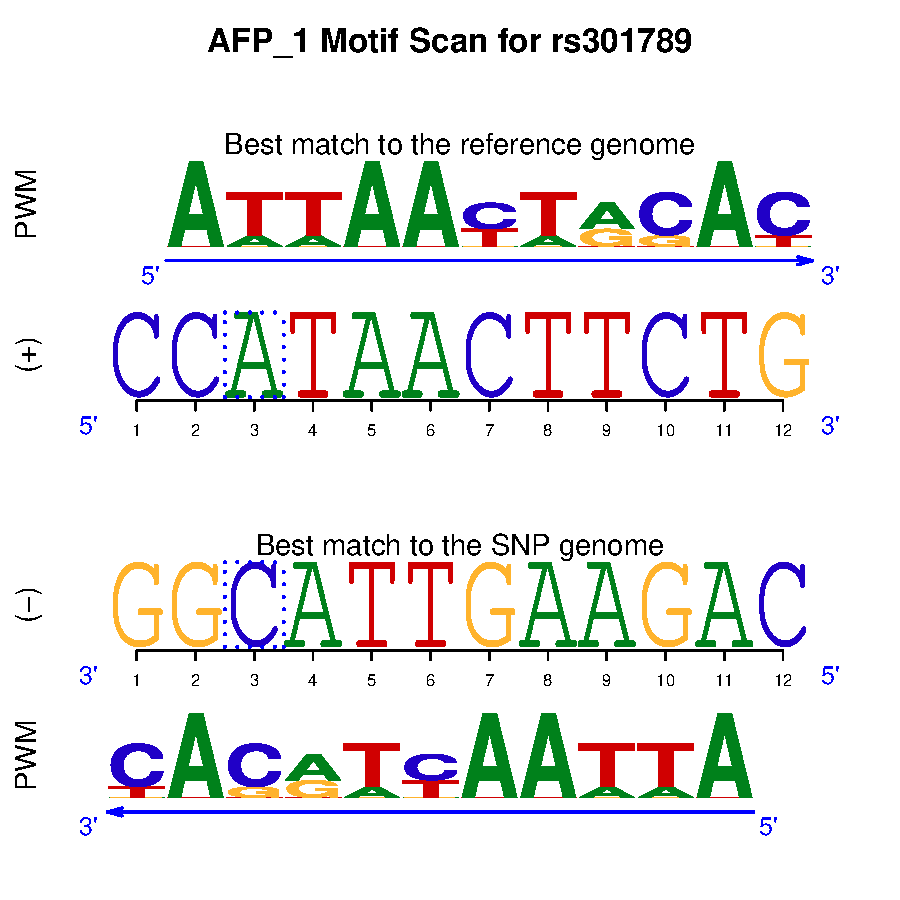
\includegraphics{atsnp-010}

\section{Session Information}

\begin{Schunk}
\begin{Soutput}
R version 3.1.1 (2014-07-10)
Platform: x86_64-redhat-linux-gnu (64-bit)

locale:
 [1] LC_CTYPE=zh_TW.UTF-8       LC_NUMERIC=C              
 [3] LC_TIME=en_US.UTF-8        LC_COLLATE=en_US.UTF-8    
 [5] LC_MONETARY=en_US.UTF-8    LC_MESSAGES=en_US.UTF-8   
 [7] LC_PAPER=en_US.UTF-8       LC_NAME=C                 
 [9] LC_ADDRESS=C               LC_TELEPHONE=C            
[11] LC_MEASUREMENT=en_US.UTF-8 LC_IDENTIFICATION=C       

attached base packages:
[1] grid      parallel  stats     graphics  grDevices utils     datasets 
[8] methods   base     

other attached packages:
 [1] atSNP_1.0          motifStack_1.6.5   ade4_1.6-2         MotIV_1.18.0      
 [5] BiocGenerics_0.8.0 grImport_0.9-0     XML_3.98-1.1       testthat_0.9.1    
 [9] doMC_1.3.3         iterators_1.0.7    foreach_1.4.2      data.table_1.9.4  
[13] Rcpp_0.11.3       

loaded via a namespace (and not attached):
 [1] Biostrings_2.30.1    BSgenome_1.30.0      chron_2.3-45        
 [4] codetools_0.2-8      compiler_3.1.1       GenomicRanges_1.14.4
 [7] IRanges_1.20.7       lattice_0.20-29      plyr_1.8.1          
[10] reshape2_1.4.1       rGADEM_2.10.0        seqLogo_1.28.0      
[13] stats4_3.1.1         stringr_0.6.2        tools_3.1.1         
[16] XVector_0.2.0       
\end{Soutput}
\end{Schunk}

\bibliographystyle{apalike}
%\bibliographystyle{natbib}

\bibliography{document}

\end{document}
